\documentclass[conference]{IEEEtran}

\usepackage[T1]{fontenc}
\usepackage[utf8]{inputenc}
\usepackage{graphicx}
\usepackage{booktabs}
\usepackage{array}
\usepackage{url}
\usepackage[hidelinks]{hyperref}
\usepackage{cite}

\title{HarmonyXR GazePose-Context: Multimodal Context Inference for Adaptive XR Training}

\author{
\IEEEauthorblockN{Varun Siddarju}
\and
\IEEEauthorblockN{Lavanya D.}
}

\begin{document}
\maketitle

\begin{abstract}
Adaptive extended reality (XR) systems require more than object interaction; they require an ability to understand whether a user is focused, distracted, transitioning between task steps, or inactive. This paper presents HarmonyXR GazePose-Context, a Unity and Meta Quest proof-of-concept that infers user context during a guided XR sorting task using runtime signals available in the current headset-facing implementation. The system follows a three-layer structure: sensor abstraction, context inference, and XR app shell adaptation. Runtime evidence was collected from a Quest headset run using Unity console logs, filtered QA evidence, processed CSV tables, and a headset video. The evidence run produced 169 QA metric samples and captured all four target context states: Engaged, Distracted, Transitioning, and Idle. The current results support the feasibility of a lightweight, interpretable adaptive XR prototype that uses multimodal runtime signals to drive user-facing guidance. Formal Phase 4 participant evaluation is currently in progress; therefore, this paper reports implementation and prototype runtime evidence rather than completed statistical user-study results.
\end{abstract}

\begin{IEEEkeywords}
extended reality, adaptive XR, context inference, gaze/AOI, hand tracking, posture, multimodal interaction, Unity, Meta Quest
\end{IEEEkeywords}

\section{Introduction}
XR training systems increasingly need to support users who shift between focused task execution, attention loss, transitional movement, and inactivity. Traditional XR applications often respond only to explicit controller input or predefined task events. This limits the system's ability to provide timely help when the user is distracted, paused, or moving between task steps.

HarmonyXR GazePose-Context addresses this problem through a lightweight multimodal context inference prototype. The system observes runtime signals from the XR scene, combines them into a shared signal frame, infers one of four user context states, and exposes adaptive support in the XR app shell. The user task is intentionally simple: sorting virtual objects into matching targets. This keeps the research focus on context inference and adaptive response rather than game complexity.

The contribution of this work is a headset-running proof-of-concept that demonstrates how multimodal XR runtime signals can support context-aware behavior during a controlled training task. The current paper is submitted as a university-ready current-version paper with Phase 4 formal evaluation still in progress.

The contributions are:
\begin{itemize}
\item a three-layer implementation structure for adaptive XR context inference;
\item a headset-facing prototype that captures gaze/AOI evidence, spatial context, hand interaction, pinch state, and gaze timing features available in the current runtime;
\item a four-state context model covering Engaged, Distracted, Transitioning, and Idle behavior;
\item a user-facing adaptive XR shell that communicates context state and task guidance; and
\item a runtime evidence package containing a headset video, console logs, filtered state evidence, and processed tables.
\end{itemize}

\section{Related Work}
\subsection{Gaze Tracking and Attention in VR}
Eye tracking is widely used in VR to estimate attention, object focus, dwell behavior, and gaze-based interaction. Moreno-Arjonilla et al. survey VR eye-tracking hardware, calibration, gaze estimation methods, datasets, and application areas, showing that gaze is a foundational signal for immersive interaction and attention analysis \cite{moreno2024eyetracking}. However, gaze-centric systems do not by themselves capture full user context because they typically do not integrate body pose, task events, or broader behavioral signals.

Pastel et al. compare gaze accuracy and precision between real-world and VR conditions \cite{pastel2021gaze}. Their results show that gaze can be useful in controlled static tasks, but accuracy and precision become more difficult under dynamic conditions. This supports the design decision in HarmonyXR GazePose-Context to avoid relying on gaze/AOI evidence alone and instead combine it with hand, posture, spatial, and task-related signals.

\subsection{Multimodal Attention and XR Interaction}
Long et al. demonstrate that multimodal physiological sensing can improve classification of internal and external attention in VR by combining EEG and eye-tracking features \cite{long2024multimodal}. This supports the broader claim that multimodal sensing can improve attention-state inference. At the same time, their approach depends on specialized EEG hardware and uses time windows that are larger than the lightweight runtime loop used in the current prototype. HarmonyXR therefore focuses on behavioral and interaction signals that can be collected inside an XR application without adding brain-computer-interface hardware.

Rakkolainen et al. provide a scoping review of multimodal interaction technologies in extended reality, covering gaze, gestures, speech, haptics, physiological sensing, and other modalities \cite{rakkolainen2021technologies}. Kim et al. later analyze the chronological shift from controller-based interaction toward hand, gaze, wrist, voice, and multimodal input across XR device generations \cite{kim2026controllers}. Together, these reviews show that XR interaction is moving toward multimodal input, but they also highlight a gap between collecting multiple input channels and using those channels for real-time behavioral context inference.

\subsection{Body, Head, and Hand Tracking}
Body and posture signals provide useful evidence about user behavior beyond visual attention. Bustamante et al. show that skeleton-based posture recognition can classify standing, sitting, and lying using lightweight geometric heuristics \cite{bustamante2025skeleton}. Neidhardt et al. show that head-mounted XR tracking can provide useful evidence about body movement during VR-based musculoskeletal training \cite{neidhardt2023body}. These works support the use of posture and movement signals, but they focus mainly on physical-state estimation rather than combining pose with gaze/AOI and task-state evidence for adaptive XR behavior.

Hand interaction is another important behavioral signal in XR because it indicates whether the user is actively manipulating or approaching task objects. Lei et al. propose a sensor-fusion approach for precise hand tracking in VR using multiple sensing sources and temporal modeling \cite{lei2023hand}. Their work focuses on improving hand-tracking accuracy, while HarmonyXR uses hand and pinch evidence as part of a higher-level context inference model.

\subsection{Gaze-Based Feedback and Context-Aware Adaptation}
Selaskowski et al. present gaze-based attention refocusing training in VR for adults with ADHD \cite{selaskowski2023gaze}. Their system uses gaze behavior to trigger feedback when attention shifts away from a continuous performance task, while also collecting EEG, head movement, and performance measures for analysis. This work is relevant because it shows how gaze behavior can drive real-time feedback, but its online decision logic remains primarily gaze-based rather than a fused multimodal context model.

Davari and Bowman propose a design space for context-aware XR interfaces and evaluate an adaptive placement strategy for XR content \cite{davari2024context}. Ramiotis and Mania propose CONTEXT-GAD, a context-aware adaptive dwell model that combines gaze behavior, head rotation, interaction frequency, and scene context to adapt gaze dwell thresholds \cite{ramiotis2025contextgad}. These works show that recent XR research is moving from gaze-only interaction toward context-aware adaptation, but the adaptation remains centered on interface placement or gaze selection rather than general user-context inference.

\subsection{Research Gap}
Existing XR research shows strong progress in gaze tracking, multimodal sensing, body/posture recognition, hand tracking, and context-aware interface adaptation. However, these strands are often treated separately: gaze systems focus on attention or selection, posture systems focus on body-state classification, hand-tracking systems focus on tracking accuracy, and context-aware XR systems often adapt placement or feedback based on narrow context definitions. HarmonyXR GazePose-Context addresses this gap at prototype level by combining runtime gaze/AOI evidence, hand interaction, posture or spatial context, and task-related signals into an interpretable four-state context model that drives adaptive XR support.

\section{Methodology}
The research problem is: how can an XR system infer user context from lightweight runtime signals and use that inference to support adaptive behavior during a training task?

The methodology follows the project implementation plan: signal acquisition, signal processing, feature extraction, multimodal fusion, context inference, and XR adaptation. The current implementation focuses on a rule-based, interpretable model rather than a black-box learning model. This decision keeps the system explainable and reproducible for the current prototype stage.

The current scope includes Unity and Meta Quest headset execution, the TrainingSimulation sorting task, four context states, runtime QA metrics, context-state evidence, and adaptive support inside the XR experience. The current scope excludes completed participant statistics, NASA-TLX results, and baseline-versus-adaptive participant comparison because Phase 4 evaluation is still in progress.

\section{System Architecture}
The implementation follows a three-layer structure: Sensor Abstraction, Context Engine, and XR App Shell. Fig.~\ref{fig:pipeline} summarizes the runtime pipeline.

\begin{figure}[t]
\centering
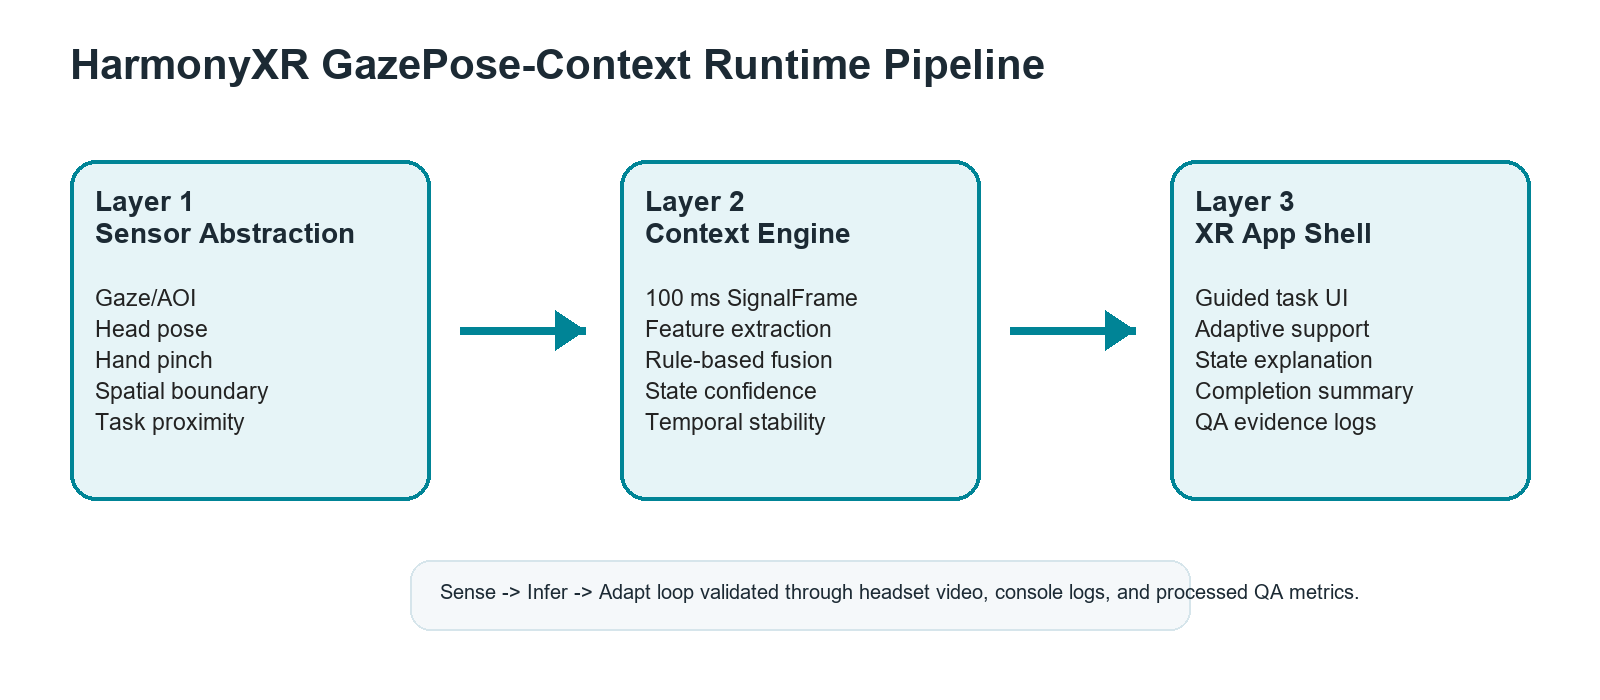
\includegraphics[width=\linewidth]{figures/figure1_runtime_pipeline.png}
\caption{HarmonyXR GazePose-Context runtime pipeline.}
\label{fig:pipeline}
\end{figure}

\subsection{Sensor Abstraction Layer}
The sensor abstraction layer converts headset and scene signals into runtime fields. Relevant fields include AOI, posture or spatial posture context, boundary mode, fixation duration, dwell ratio, saccade rate, body activity, hand interaction count, pinch state, and distance to task object. These fields are emitted through QA metrics and logged for validation.

\subsection{Context Engine}
The context engine consumes synchronized runtime evidence and infers a context state. The current implementation uses interpretable rule-based logic and confidence values. The system infers four runtime states: Engaged, Distracted, Transitioning, and Idle.

\subsection{XR App Shell}
The XR app shell translates inferred state into visible user support. It includes onboarding, task guidance, context-aware feedback, adaptive support actions, QA/evidence logging, and end-of-session completion messaging.

\section{Prototype Implementation}
The prototype is implemented in Unity and has been migrated to Unity 6000.4.7f1 for the current submission build. The verified Quest build uses OpenXR 1.16.1, Meta XR Core SDK 201.0.0, and URP 17.4.0. The app targets Meta Quest headset execution. The primary scene is TrainingSimulation, where the user sorts a cube, cylinder, and sphere into corresponding pads or receptacles.

The main implementation components are:
\begin{itemize}
\item \textbf{SignalSynchroniser}: emits runtime signal frames on a 100 ms cadence.
\item \textbf{ContextDebugTester / context pipeline}: evaluates context state and confidence.
\item \textbf{TrainingSimulationUserGuide}: presents onboarding, task guidance, incorrect-object messaging, and completion summary.
\item \textbf{AdaptationManager}: maps inferred context states to adaptive XR support and QA metric console logging.
\item \textbf{ContextLogger}: records context output for analysis.
\end{itemize}

The proof-of-concept intentionally stays within a narrow research scope. It does not add unrelated gameplay or study-management systems. The goal is to show that adaptive XR behavior can be driven by inferred context signals during a simple task.

\section{Context State Model}
The system infers four context states:
\begin{itemize}
\item \textbf{Engaged}: focused on task-relevant content or interacting with the current task.
\item \textbf{Distracted}: attention shifted away from the task or task-directed activity reduced.
\item \textbf{Transitioning}: movement between task steps, targets, or interaction states.
\item \textbf{Idle}: low activity, little interaction, or a pause state.
\end{itemize}
These states are runtime categories for adaptive behavior and evidence reporting. They are not clinical or psychological diagnoses.

\section{Evidence Collection and Current Results}
Evidence was collected through a combined headset evidence run on May 14, 2026. ADB logcat captured Unity runtime console output while the application ran in the Quest headset. The collected artifacts were organized under \texttt{Research\_Evidence}.

Primary evidence files include the full headset evidence video, raw console evidence, filtered console evidence, QA metrics CSV, state coverage table, adaptation event table, and stability table. The evidence run produced 169 QA metric samples. Each QA metric line contained state, confidence, boundary, AOI, posture/spatial context, fixation, dwell, saccade, body activity, hand interaction count, pinch state, and distance to task object.

\subsection{Context State Coverage}
All four required context states appeared in the headset evidence run. Table~\ref{tab:statecoverage} reports the observed state counts.

\begin{table}[t]
\centering
\caption{Context state coverage from headset runtime evidence.}
\label{tab:statecoverage}
\begin{tabular}{lrr}
\toprule
State & Samples & Found \\
\midrule
Engaged & 15 & Yes \\
Distracted & 30 & Yes \\
Transitioning & 100 & Yes \\
Idle & 24 & Yes \\
\bottomrule
\end{tabular}
\end{table}

\begin{figure}[t]
\centering
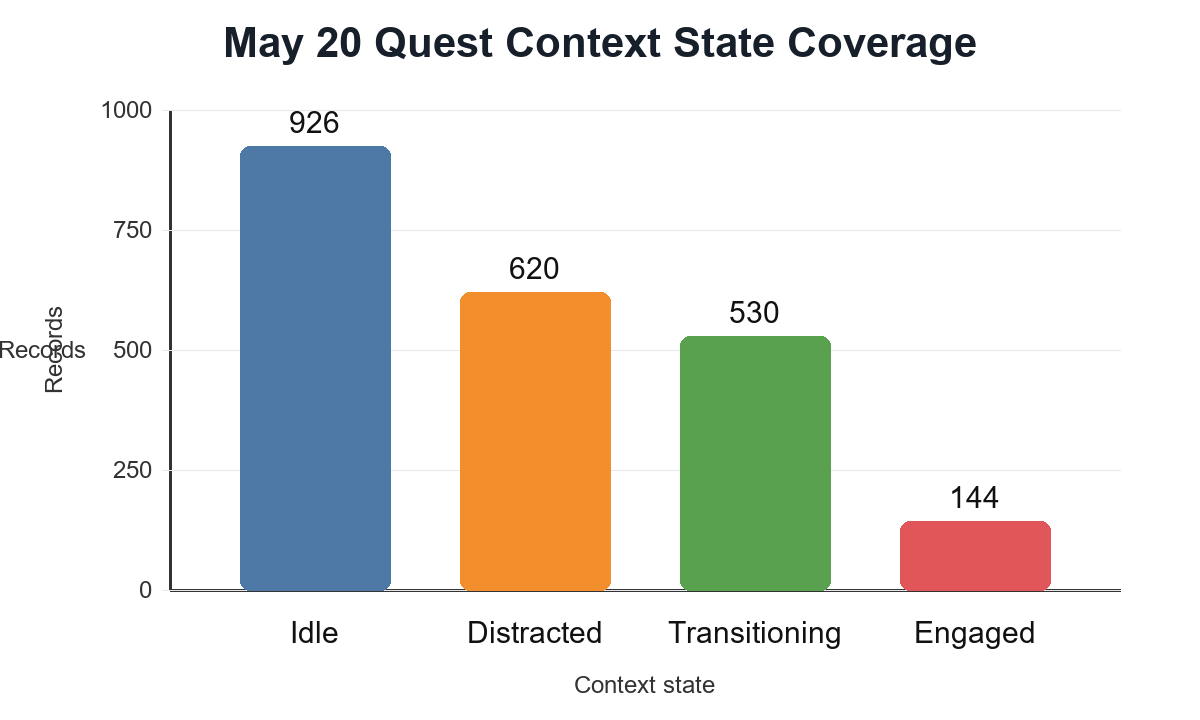
\includegraphics[width=\linewidth]{figures/figure2_state_coverage.png}
\caption{Context state sample counts observed in the headset evidence run.}
\label{fig:coverage}
\end{figure}

\subsection{Runtime Signal Coverage}
The QA metric log confirms that the runtime emitted the key signal fields required for paper evidence: AOI, POSTURE, BOUND, FIX, DWELL, SACC, BODY, HAND, PINCH, and DIST. These fields were present in the runtime console log and in the processed \texttt{qa\_metrics\_extract.csv} table.

\subsection{Adaptive Behavior Evidence}
The adaptation evidence table records each trigger state and its expected adaptive response category. Engaged maps to normal task support, Distracted maps to refocus or attention guidance, Transitioning maps to soft movement or task-step support, and Idle maps to pause or adaptive support behavior. The current evidence shows that the trigger states are emitted during headset runtime. Visual confirmation is supported by the full headset evidence video. This evidence should be interpreted as runtime behavior proof, not as a controlled measurement of user benefit.

\subsection{Stability Evidence}
The run captured QA metric output from 05-14 16:16:46.104 through 05-14 16:22:02.470. No crash was indicated in the captured evidence, and the QA metric stream continued during the run. The available evidence therefore supports runtime continuity during the captured session. A more detailed latency analysis with explicit measured values should be added before making a strong real-time performance claim.

\section{Evaluation Status}
Formal Phase 4 evaluation is currently in progress. Therefore, this paper does not claim completed participant results, statistical significance, NASA-TLX findings, or a completed baseline-versus-adaptive user-study comparison.

The planned Phase 4 evaluation is expected to compare baseline and adaptive conditions and collect task completion time, sorting errors, context detection accuracy against ground truth, and subjective workload. These outputs are not reported as completed results in the current submission.

\section{Discussion}
The evidence supports the central claim that a headset-running XR prototype can infer and expose user context using lightweight multimodal runtime signals. The presence of all four context states demonstrates that the model is reachable across expected behavioral conditions. This does not by itself prove classification accuracy because no participant ground truth or independent annotation is included in the current evidence package. The signal coverage table demonstrates that the runtime records enough evidence to support analysis of gaze/AOI, posture or spatial posture context, hand interaction, pinch state, and gaze-derived timing features.

The communication improvements in the app shell are also important. Earlier versions of the prototype risked appearing like a technical debug demo. The current presentation better explains the research purpose, active task, inferred state, and adaptive support. This matters because the proof-of-concept is intended for first-time users, clients, and research stakeholders, not only developers.

\section{Limitations}
This work remains a prototype-level validation rather than a completed user study. The evidence comes from a headset evidence run, not from a multi-participant controlled experiment. The results should therefore be interpreted as proof-of-concept validation, not as statistical evidence that adaptive XR improves task performance or workload.

Several implementation boundaries should be noted. The current paper uses gaze/AOI evidence as recorded by the runtime and does not claim a completed participant-calibrated eye-tracking accuracy study. The \texttt{room\_scale} posture value should be interpreted as spatial or boundary context, not strict sitting/standing recognition. Sitting or standing should only be discussed where explicit sitting or standing values appear in the logs. The current context log format is JSONL-style runtime evidence rather than a single JSON array document. Guide-level QA requirements such as formal participant self-report ground truth and baseline/adaptive comparisons remain Phase 4 work.

\section{Conclusion}
HarmonyXR GazePose-Context demonstrates a working adaptive XR proof-of-concept that infers user context from runtime signals and uses that context to support task guidance. The headset evidence package confirms all four target states and 169 QA metric samples containing key signal fields. While formal Phase 4 participant evaluation remains in progress, the current implementation provides a credible systems prototype and evidence base for an adaptive XR research paper.

\section*{Acknowledgment and Disclosure}
This paper was prepared from the current OpenSpatialAI implementation, HarmonyXR planning documents, and the May 14, 2026 evidence package. All implementation details, evidence, technical claims, and final content were reviewed and verified by the authors.

\begin{thebibliography}{11}

\bibitem{moreno2024eyetracking}
J. Moreno-Arjonilla, A. Lopez-Ruiz, J. R. Jimenez-Perez, J. E. Callejas-Aguilera, and J. M. Jurado, ``Eye-tracking on virtual reality: a survey,'' \emph{Virtual Reality}, vol. 28, article 38, 2024, doi: 10.1007/s10055-023-00903-y.

\bibitem{pastel2021gaze}
S. Pastel, C.-H. Chen, L. Martin, M. Naujoks, K. Petri, and K. Witte, ``Comparison of gaze accuracy and precision in real-world and virtual reality,'' \emph{Virtual Reality}, vol. 25, pp. 175--189, 2021, doi: 10.1007/s10055-020-00449-3.

\bibitem{long2024multimodal}
X. Long, S. Mayer, and F. Chiossi, ``Multimodal detection of external and internal attention in virtual reality using EEG and eye tracking features,'' in \emph{Proceedings of Mensch und Computer 2024 (MuC '24)}, 2024, doi: 10.1145/3670653.3670657.

\bibitem{rakkolainen2021technologies}
I. Rakkolainen, A. Farooq, J. Kangas, J. Hakulinen, J. Rantala, M. Turunen, and R. Raisamo, ``Technologies for multimodal interaction in extended reality: a scoping review,'' \emph{Multimodal Technologies and Interaction}, vol. 5, no. 12, article 81, 2021, doi: 10.3390/mti5120081.

\bibitem{kim2026controllers}
H. Kim, S. Lee, and C. Kang, ``From controllers to multimodal input: a chronological review of XR interaction across device generations,'' \emph{Sensors}, vol. 26, no. 1, article 196, 2026, doi: 10.3390/s26010196.

\bibitem{bustamante2025skeleton}
A. Bustamante, L. M. Belmonte, A. Pereira, R. Morales, and A. Fernandez-Caballero, ``Skeleton-based posture recognition for home care from virtual unmanned aerial vehicle,'' \emph{Expert Systems}, 2025, doi: 10.1111/exsy.70108.

\bibitem{neidhardt2023body}
M. Neidhardt, S. Gerlach, F. N. Schmidt, I. A. K. Fiedler, S. Grube, B. Busse, and A. Schlaefer, ``VR-based body tracking to stimulate musculoskeletal training,'' arXiv:2308.03375, 2023.

\bibitem{lei2023hand}
Y. Lei, Y. Deng, L. Dong, X. Li, X. Li, and Z. Su, ``A novel sensor fusion approach for precise hand tracking in virtual reality-based human-computer interaction,'' \emph{Biomimetics}, vol. 8, no. 3, article 326, 2023, doi: 10.3390/biomimetics8030326.

\bibitem{selaskowski2023gaze}
B. Selaskowski \emph{et al.}, ``Gaze-based attention refocusing training in virtual reality for adult attention-deficit/hyperactivity disorder,'' \emph{BMC Psychiatry}, vol. 23, article 74, 2023, doi: 10.1186/s12888-023-04551-z.

\bibitem{davari2024context}
S. Davari and D. A. Bowman, ``Towards context-aware adaptation in extended reality: a design space for XR interfaces and an adaptive placement strategy,'' arXiv:2411.02607, 2024, doi: 10.48550/arXiv.2411.02607.

\bibitem{ramiotis2025contextgad}
G. Ramiotis and K. Mania, ``CONTEXT-GAD: a context-aware gaze adaptive dwell model for gaze-based selections in XR environments,'' in \emph{Proceedings of the 31st ACM Symposium on Virtual Reality Software and Technology (VRST '25)}, 2025, doi: 10.1145/3756884.3766048.

\end{thebibliography}

\end{document}
